\documentclass[10pt,a4paper]{article}
\usepackage[utf8]{inputenc}
\usepackage{amsmath}
\usepackage{amsfonts}
\usepackage{amssymb}
\usepackage{tikz}
\usepackage{graphicx}
\author{James Lee}
\title{12th Assignment of Computational Physics}
\begin{document}
	\maketitle
	\begin{abstract}
		In this report I present to you the numerical solution to Problem 4.16.
	\end{abstract}
	\section{Introduction}
	In physics and classical mechanics, the three-body problem is the problem of taking an initial set of data that specifies the positions, masses and velocities of three bodies for some particular point in time and then determining the motions of the three bodies, in accordance with the laws of classical mechanics (Newton's laws of motion and of universal gravitation). The three-body problem is a special case of the n-body problem.\\
	The gravitational problem of three bodies in its traditional sense dates in substance from 1687, when Isaac Newton published his "Principia" (Philosophiæ Naturalis Principia Mathematica). In Proposition 66 of Book 1 of the "Principia", and its 22 Corollaries, Newton took the first steps in the definition and study of the problem of the movements of three massive bodies subject to their mutually perturbing gravitational attractions. In Propositions 25 to 35 of Book 3, Newton also took the first steps in applying his results of Proposition 66 to the lunar theory, the motion of the Moon under the gravitational influence of the Earth and the Sun.\\
	The problem became of technical importance in the 1720s, as an accurate solution would be applicable to navigation, specifically for the determination of longitude at sea. This problem was addressed by Amerigo Vespucci and by Galileo Galilei before being solved by John Harrison's invention of the Marine chronometer. Before the chronometer became available, Vespucci had used, in 1499, knowledge of the position of the moon to determine his position in Brazil. However the accuracy of the lunar theory was low, due to the perturbing effect of the Sun, and planets, on the motion of the Moon around the Earth.\\
	Jean d'Alembert and Alexis Clairaut, who developed a longstanding rivalry, both attempted to analyze the problem in some degree of generality, and by the use of differential equations to be solved by successive approximations. They submitted their competing first analyses to the Académie Royale des Sciences in 1747.\\
	It was in connection with these researches, in Paris, in the 1740s, that the name "three-body problem" (Problème des Trois Corps) began to be commonly used. An account published in 1761 by Jean d'Alembert indicates that the name was first used in 1747.\\
	In 1887, mathematicians Heinrich Bruns and Henri Poincaré showed that there is no general analytical solution for the three-body problem given by algebraic expressions and integrals. The motion of three bodies is generally non-repeating, except in special cases.\\
	After having proposed the theory of general relativity, Einstein showed that general relativity agrees closely with the observed amount of perihelion shift. This was a powerful factor motivating the adoption of general relativity.\\
	In the following discussions, I will consider Sun-Earth-Jupiter system and further assume that their orbits are in the same plane.\\
	The ODE set that governs the evolution is:
	\begin{align}
	\frac{dx_s}{dt}&=v_{sx}\\
	\frac{dy_s}{dt}&=v_{sy}\\
	\frac{dx_j}{dt}&=v_{jx}\\
	\frac{dy_j}{dt}&=v_{jy}\\
	\frac{dx_e}{dt}&=v_{ex}\\
	\frac{dy_e}{dt}&=v_{ey}\\
	\frac{dv_{sx}}{dt}&=\frac{GM_e(x_e-x_s)}{r_{es}^3}+\frac{GM_j(x_j-x_s)}{r_{js}^3}\\
	\frac{dv_{sy}}{dt}&=\frac{GM_e(y_e-y_s)}{r_{es}^3}+\frac{GM_j(y_j-y_s)}{r_{js}^3}\\
	\frac{dv_{jx}}{dt}&=\frac{GM_e(x_e-x_j)}{r_{ej}^3}+\frac{GM_s(x_s-x_j)}{r_{sj}^3}\\
	\frac{dv_{jy}}{dt}&=\frac{GM_e(y_e-y_j)}{r_{ej}^3}+\frac{GM_s(y_s-y_j)}{r_{sj}^3}\\
	\frac{dv_{ex}}{dt}&=\frac{GM_s(x_s-x_e)}{r_{se}^3}+\frac{GM_j(x_j-x_e)}{r_{je}^3}\\
	\frac{dv_{ey}}{dt}&=\frac{GM_s(y_s-y_e)}{r_{se}^3}+\frac{GM_j(y_j-y_e)}{r_{je}^3}
	\end{align}
	where
	\begin{align}
	r_{se}&=r_{es}=\sqrt{(x_s-x_e)^2+(y_s-y_e)^2}\\
	r_{sj}&=r_{js}=\sqrt{(x_s-x_j)^2+(y_s-y_j)^2}\\
	r_{je}&=r_{ej}=\sqrt{(x_j-x_e)^2+(y_j-y_e)^2}\\
	\end{align}
	Clearly, this set of ODE is hard to solve.\\
	In the following sections, I will use numerical methods to study the subject.
	
    \section{Main Content}
    \subsection{Real Initial Conditions}
    Set the initial conditions as the real values:
    \begin{align}
    x_e|_{t=0}&=1\text{ AU}\\
    y_e|_{t=0}&=0\\
    v_{ex}|_{t=0}&=0\\
    v_{ey}|_{t=0}&=2\pi\text{ AU/Yr}\\
    x_j|_{t=0}&=5.2\text{ AU}\\
    y_j|_{t=0}&=0\\
    v_{jx}|_{t=0}&=0\\
    v_{jy}|_{t=0}&=2\pi\frac{5.2}{11.86}\text{ AU/Yr}=0.877\pi\text{ AU/Yr}\\
    x_s|_{t=0}&=0\\
    y_s|_{t=0}&=0\\
    v_{sx}|_{t=0}&=0\\
    v_{sy}|_{t=0}&=0
    \end{align}
    With the dynamical equations and initial conditions in hands, one can easily obtain the orbit.\\
    \begin{figure}[htbp]
    	\centering
    	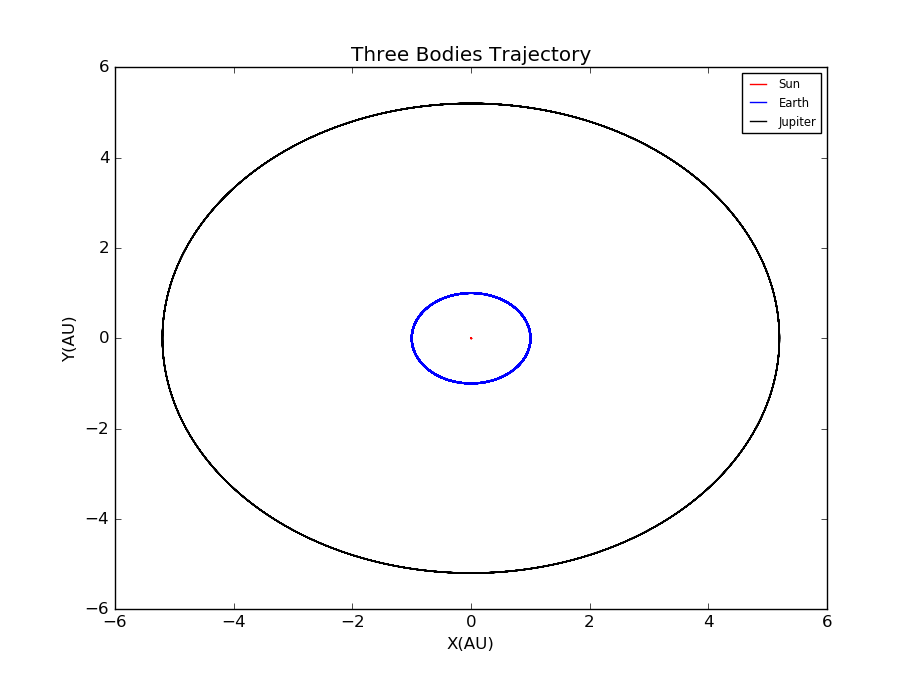
\includegraphics[width=5in]{threebodies_1.png}
    	\caption{Three Bodies Trajectory with Real Initial Condition}
    \end{figure}
    I should remark that this program is run under 100 years.\\
    As we can see in the plot, real intial conditions produce stable and closed orbits, which are just we expected.
    \subsection{Different Initial Conditions}
    Here below I list some of the interesting cases:
    \begin{figure}[htbp]
    	\centering
    	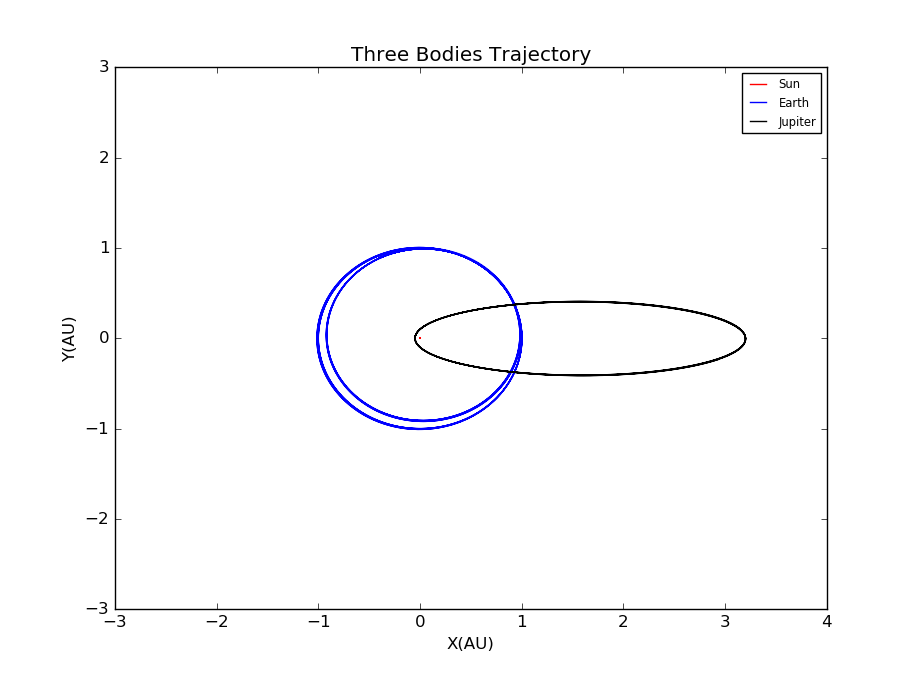
\includegraphics[width=5in]{threebodies_2.png}
    	\caption{Three Bodies Trajectory with $x_j=3.2, v_{jy}=0.2\pi$}
    \end{figure}
   \begin{figure}[htbp]
   	\centering
   	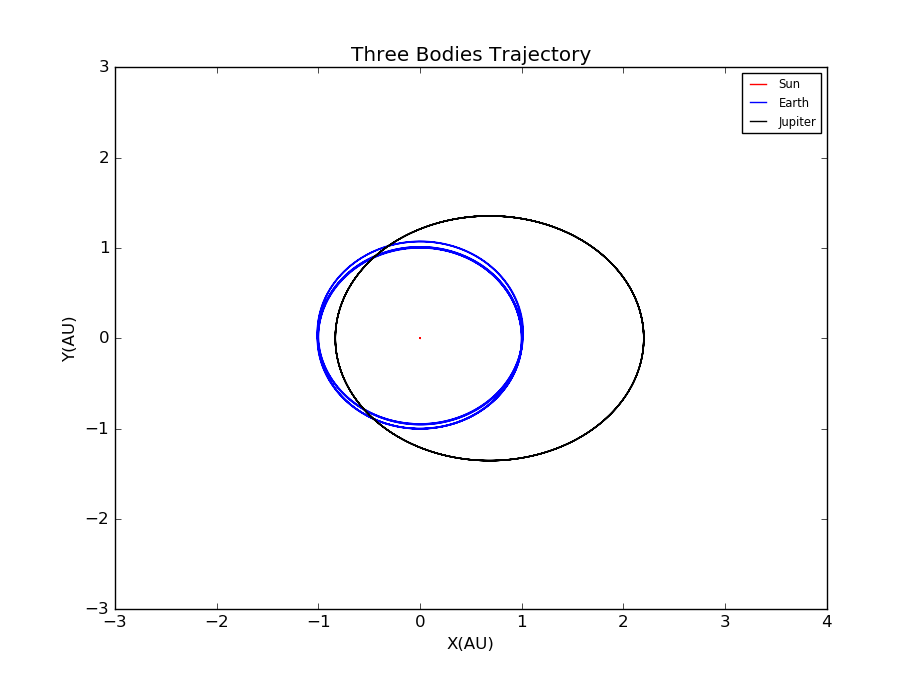
\includegraphics[width=5in]{threebodies_3.png}
   	\caption{Three Bodies Trajectory with $x_j=2.2, v_{jy}=\pi$}
   \end{figure}
    \begin{figure}[htbp]
    	\centering
    	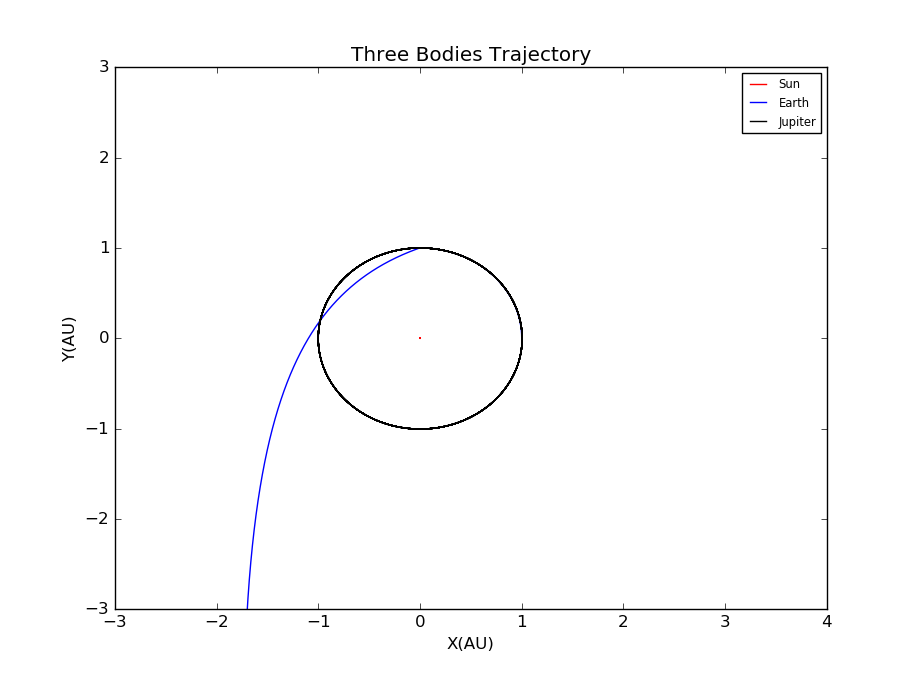
\includegraphics[width=5in]{threebodies_4.png}
    	\caption{Three Bodies Trajectory with $x_j=-1, v_{jy}=2\pi$}
    \end{figure}
    We should notice that in several cases, the orbits are unstable in time.
    
    \subsection{Different Jupiter Mass}
    Now we set the initial values as the real values, and set Jupiter's mass as different values.\\
    \begin{figure}[htbp]
    	\centering
    	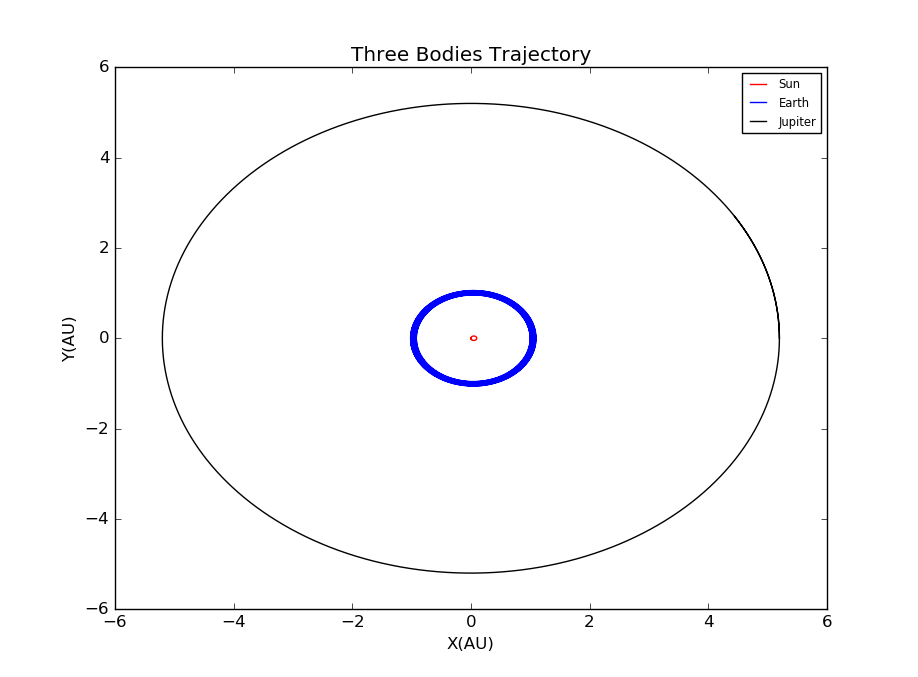
\includegraphics[width=5in]{threebodies_5.png}
    	\caption{Three Bodies Trajectory with $M_J=10M_{J,real}$}
    \end{figure}
    \begin{figure}[htbp]
    		\centering
    		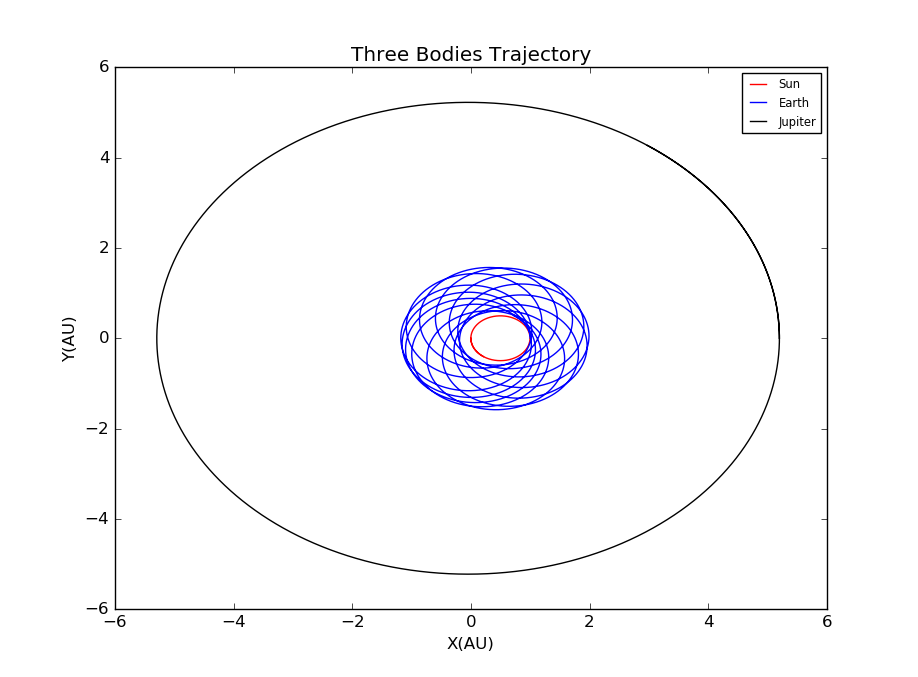
\includegraphics[width=5in]{threebodies_6.png}
    		\caption{Three Bodies Trajectory with $M_J=100M_{J,real}$}
    \end{figure}
    \begin{figure}[htbp]
    	\centering
    	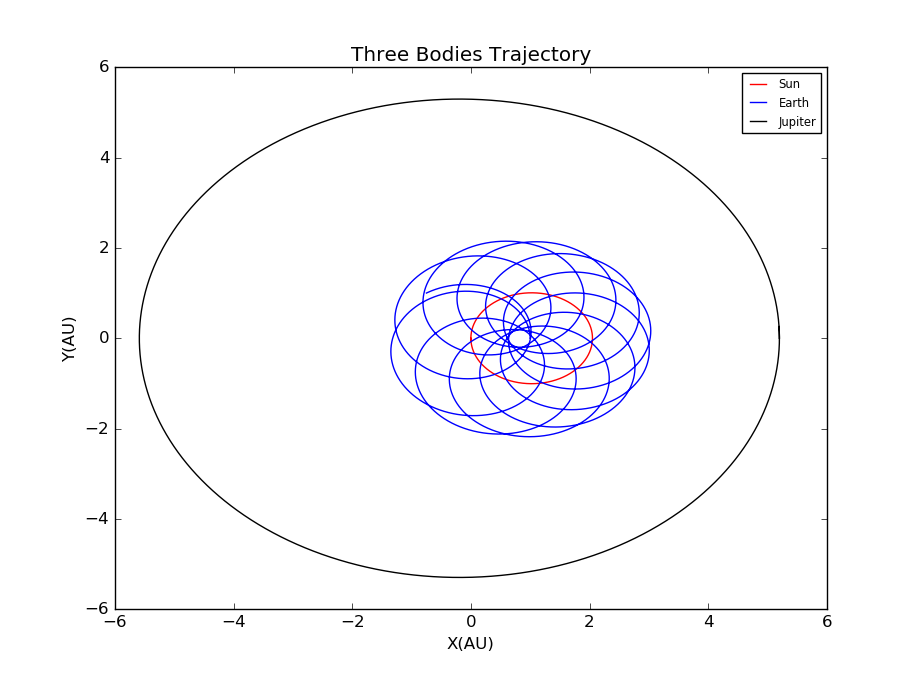
\includegraphics[width=5in]{threebodies_8.png}
    	\caption{Three Bodies Trajectory with $M_J=200M_{J,real}$}
    \end{figure}
    \begin{figure}[htbp]
    	\centering
    	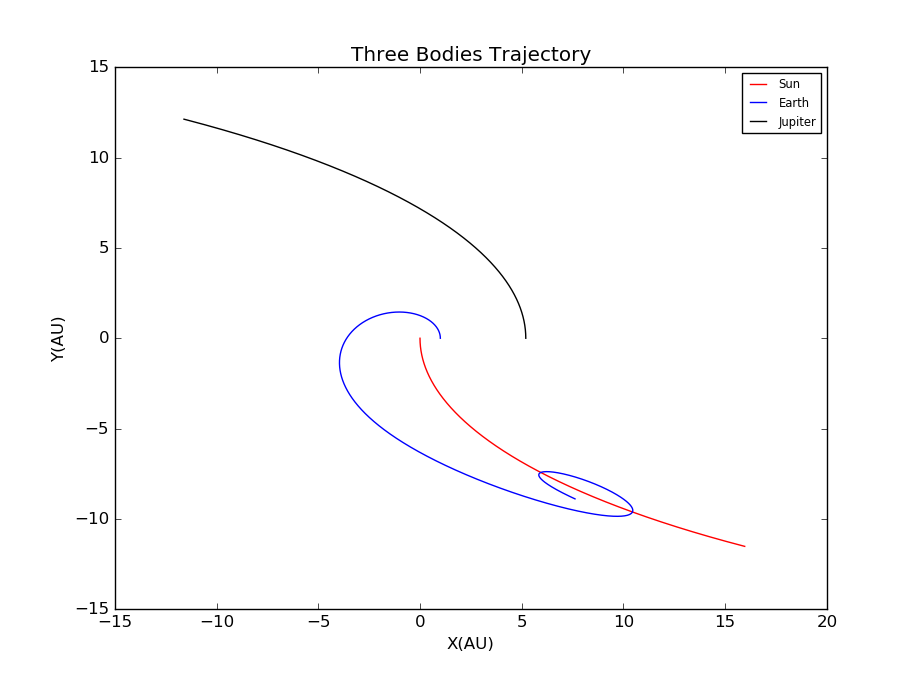
\includegraphics[width=5in]{threebodies_7.png}
    	\caption{Three Bodies Trajectory with $M_J=1000M_{J,real}$}
    \end{figure}
    As Jupiter's mass increases, Sun begins to moves in a larger and larger circle, and earth's orbit becomes unstable. Eventually, earth will get ejected out of the system.\\
    Three body system is quite common in the universe, we are lucky to live in a stable system.
\end{document}